% l = 8

\begin{figure}[H]
\begin{center}
\subfloat{
\resizebox{8cm}{5cm}{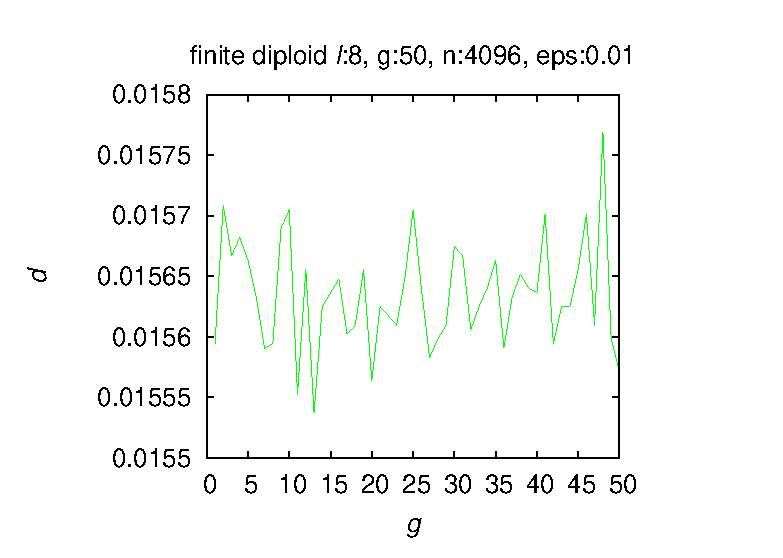
\includegraphics{figures/eps/vio/mu/b8/e0.01/n00004096_fin_dip.eps}}}\hspace{-3em}%
\subfloat{
\resizebox{8cm}{5cm}{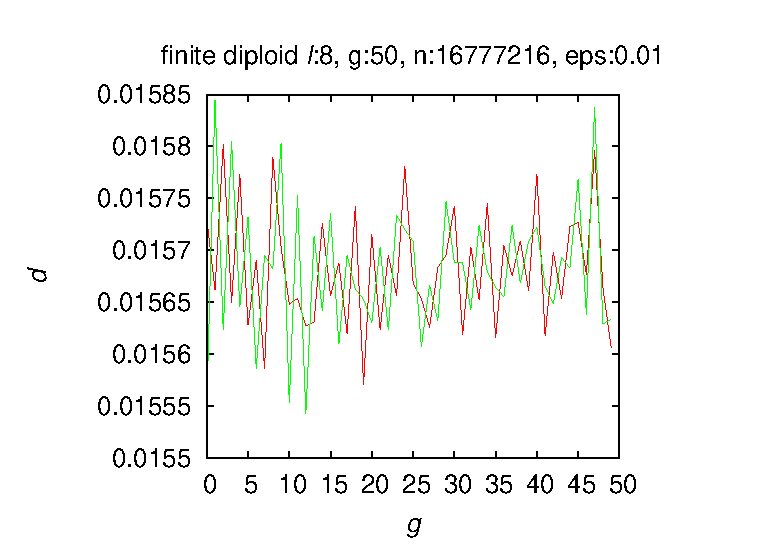
\includegraphics{figures/eps/vio/mu/b8/e0.01/n00004096_fin_dip_wovio.eps}}}\vspace{-1em}  \hspace{-3em}%
\end{center}
\begin{center}
\subfloat{
\resizebox{8cm}{5cm}{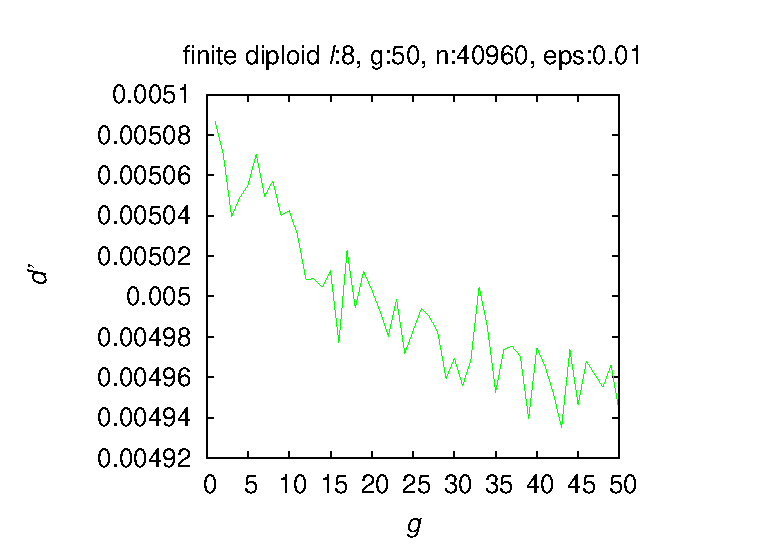
\includegraphics{figures/eps/vio/mu/b8/e0.01/n00040960_fin_dip.eps}}}\hspace{-3em}%
\subfloat{
\resizebox{8cm}{5cm}{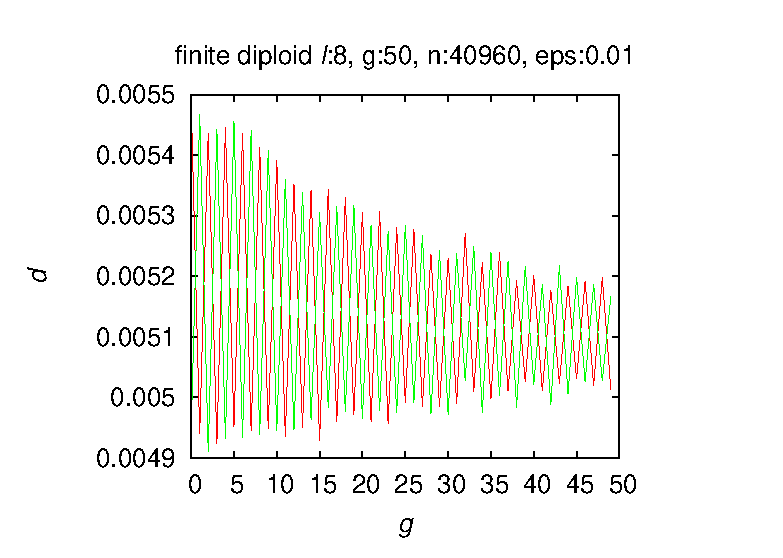
\includegraphics{figures/eps/vio/mu/b8/e0.01/n00040960_fin_dip_wovio.eps}}}\vspace{-1em}  \hspace{-3em}%
\end{center}


\begin{center}
\subfloat{
\resizebox{8cm}{5cm}{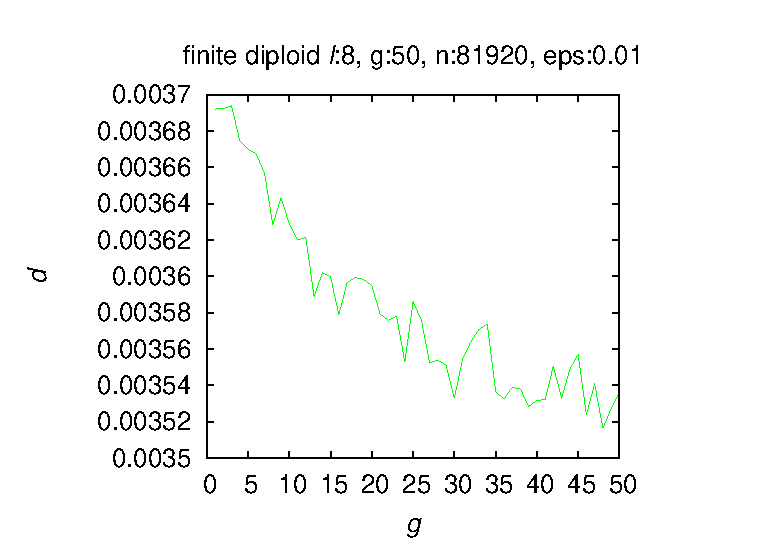
\includegraphics{figures/eps/vio/mu/b8/e0.01/n00081920_fin_dip.eps}}}\hspace{-3em}%
\subfloat{
\resizebox{8cm}{5cm}{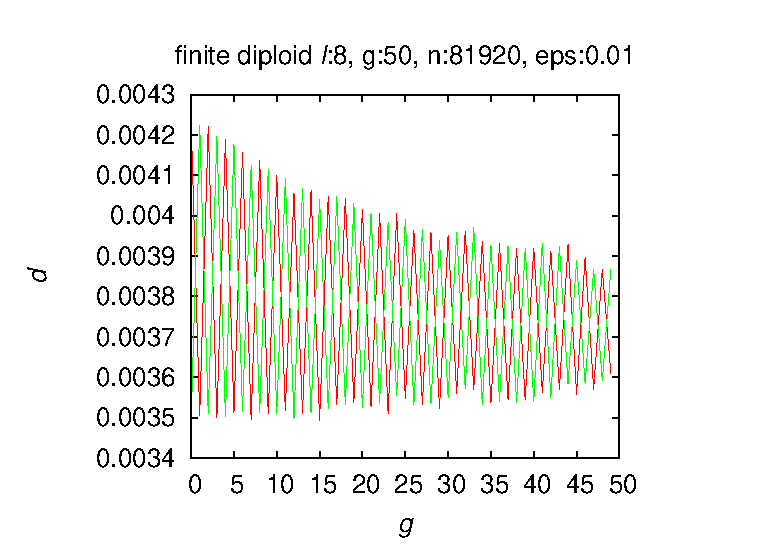
\includegraphics{figures/eps/vio/mu/b8/e0.01/n00081920_fin_dip_wovio.eps}}}\vspace{-1em}  \hspace{-3em}%
\end{center}

\begin{center}
\subfloat{
\resizebox{8cm}{5cm}{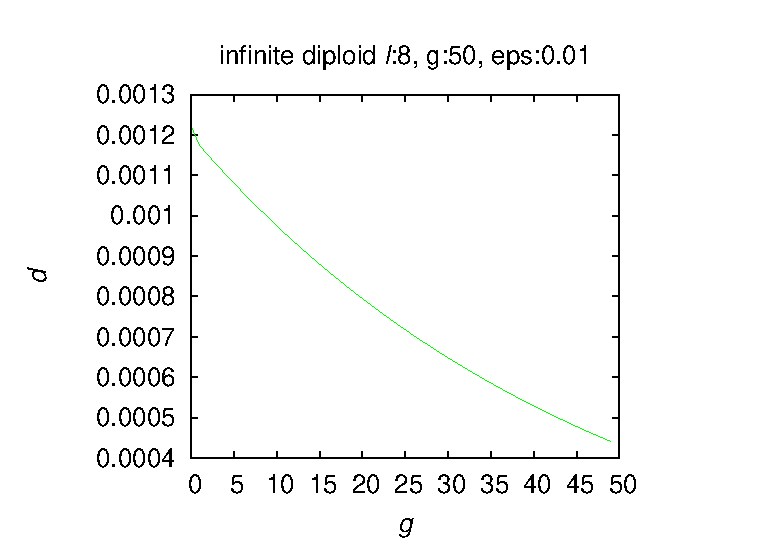
\includegraphics{figures/eps/vio/mu/b8/e0.01/inf_dip.eps}}}\hspace{-3em}%
\subfloat{
\resizebox{8cm}{5cm}{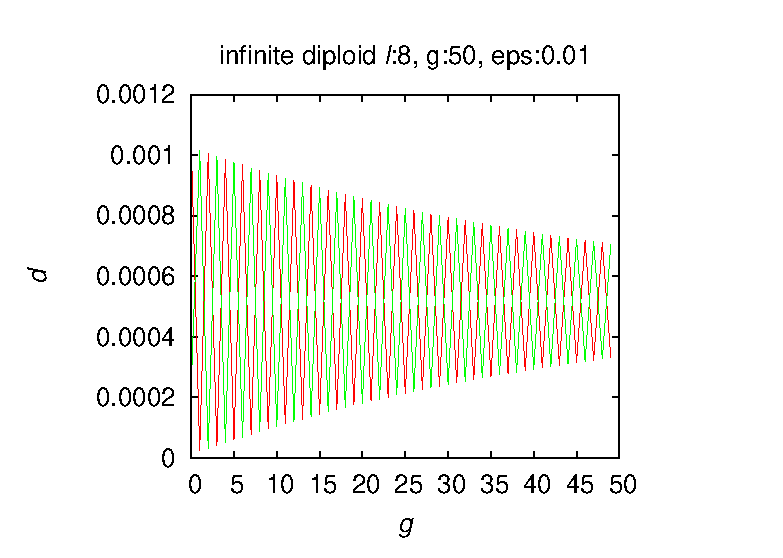
\includegraphics{figures/eps/vio/mu/b8/e0.01/inf_dip_wovio.eps}}}\vspace{-0.5em}  \hspace{-3em}%


\caption{\textbf{Infinite and finite diploid population oscillation behavior in case of violation in $\bm{\mu}$ for genome length $\ell = 8$ and $\bm{\epsilon} = 0.01$:} 
  In left column, $d'$ is distance of finite population of size $n$ or infinite population to limit $\bm{z}^\ast$ for $g$ generations. In right column, $d$ is distance of finite population of size $N$ or infinite population to limits without violation.}
\label{oscillation_8d_vio_mu_0.01}
\end{center}
\end{figure}

% l = 10

\begin{figure}[H]
\begin{center}
\subfloat{
\resizebox{8cm}{5cm}{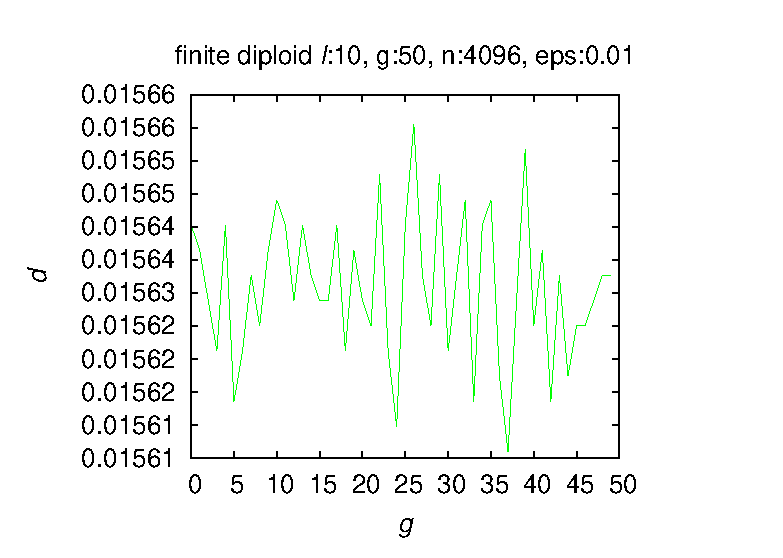
\includegraphics{figures/eps/vio/mu/b10/e0.01/n00004096_fin_dip.eps}}}\hspace{-3em}%
\subfloat{
\resizebox{8cm}{5cm}{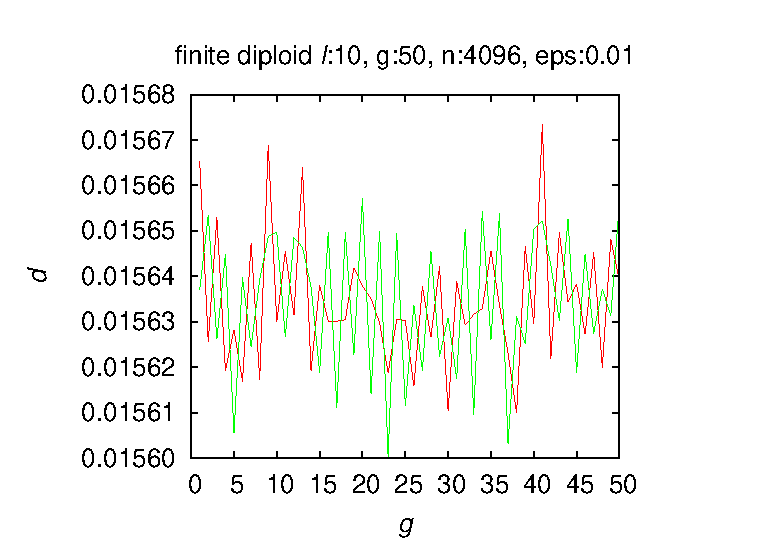
\includegraphics{figures/eps/vio/mu/b10/e0.01/n00004096_fin_dip_wovio.eps}}}\vspace{-1em}  \hspace{-3em}%
\end{center}
\begin{center}
\subfloat{
\resizebox{8cm}{5cm}{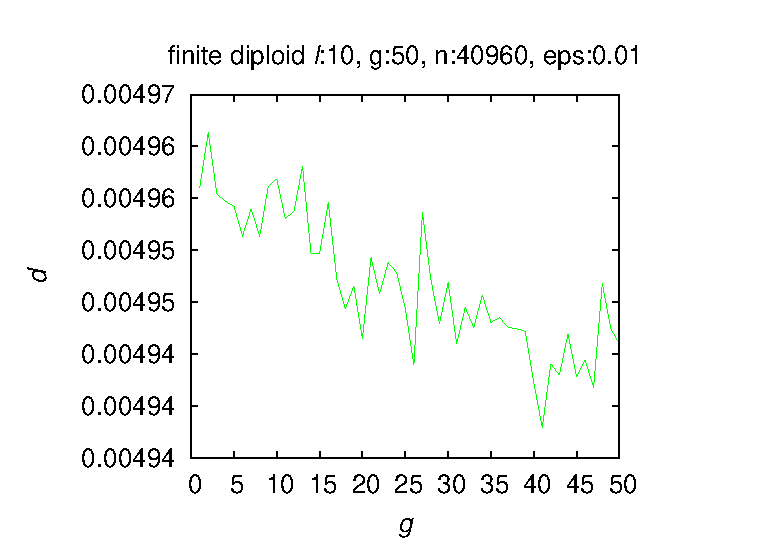
\includegraphics{figures/eps/vio/mu/b10/e0.01/n00040960_fin_dip.eps}}}\hspace{-3em}%
\subfloat{
\resizebox{8cm}{5cm}{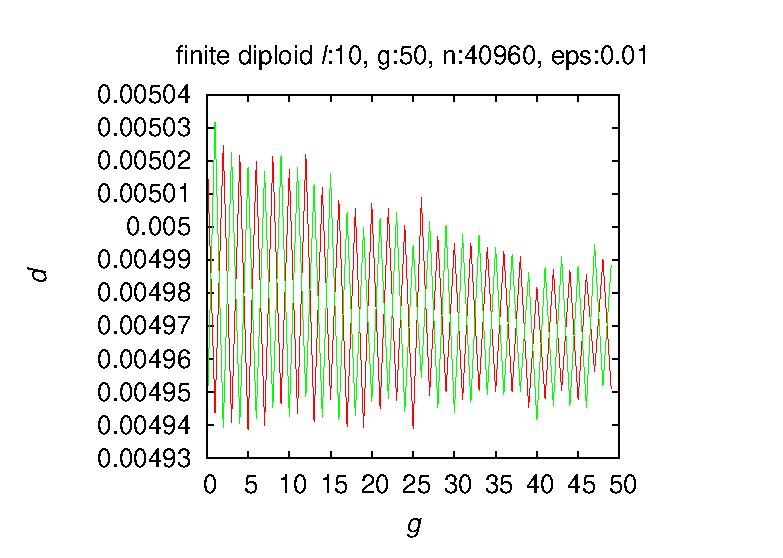
\includegraphics{figures/eps/vio/mu/b10/e0.01/n00040960_fin_dip_wovio.eps}}}\vspace{-1em}  \hspace{-3em}%
\end{center}


\begin{center}
\subfloat{
\resizebox{8cm}{5cm}{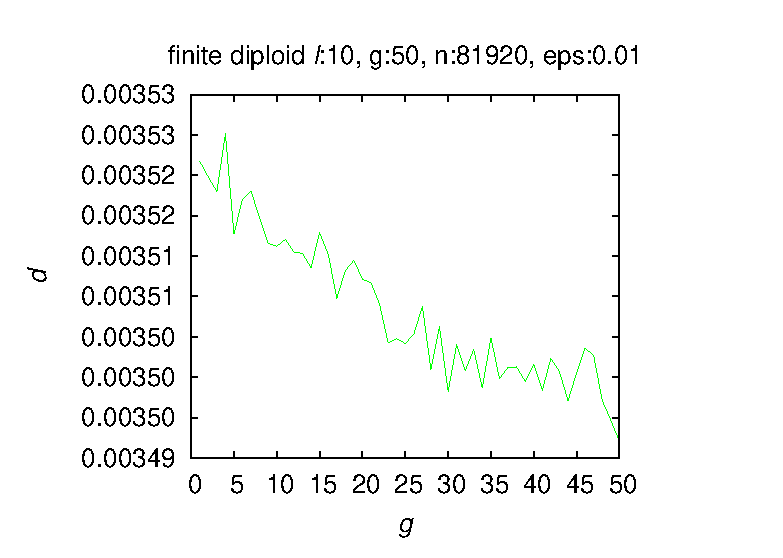
\includegraphics{figures/eps/vio/mu/b10/e0.01/n00081920_fin_dip.eps}}}\hspace{-3em}%
\subfloat{
\resizebox{8cm}{5cm}{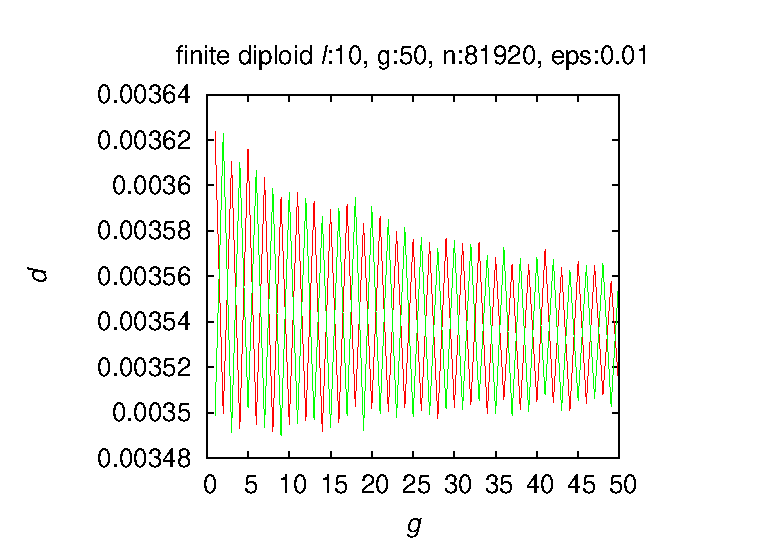
\includegraphics{figures/eps/vio/mu/b10/e0.01/n00081920_fin_dip_wovio.eps}}}\vspace{-1em}  \hspace{-3em}%
\end{center}

\begin{center}
\subfloat{
\resizebox{8cm}{5cm}{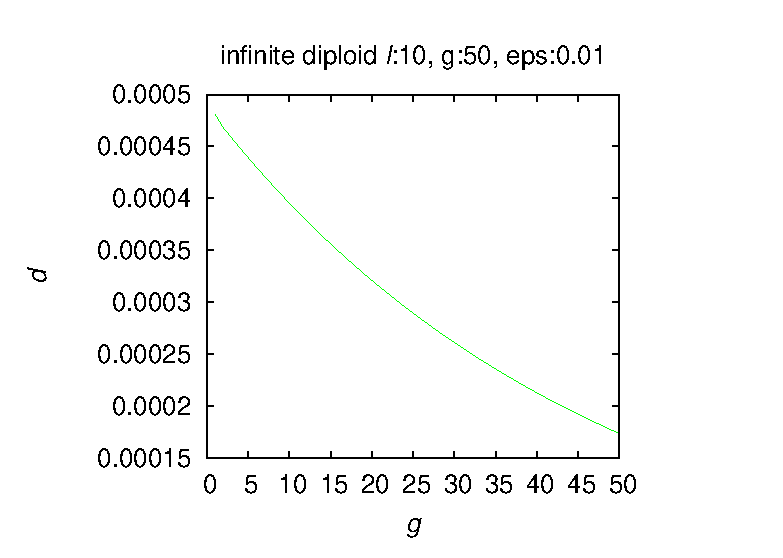
\includegraphics{figures/eps/vio/mu/b10/e0.01/inf_dip.eps}}}\hspace{-3em}%
\subfloat{
\resizebox{8cm}{5cm}{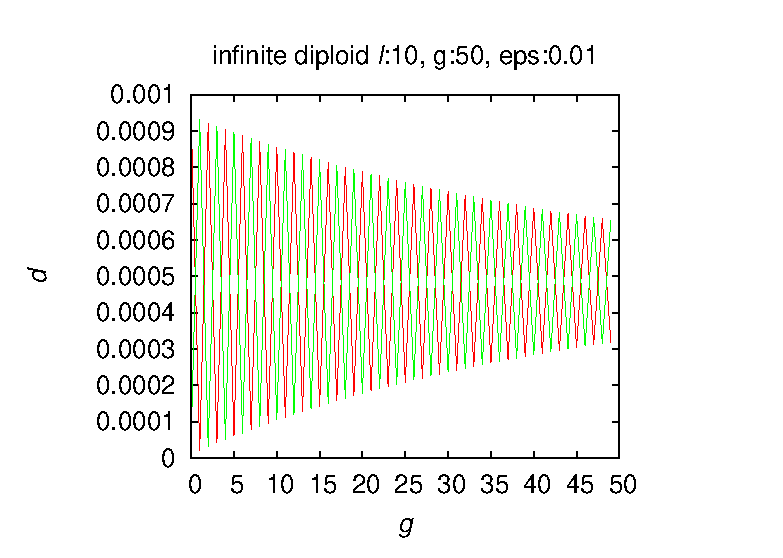
\includegraphics{figures/eps/vio/mu/b10/e0.01/inf_dip_wovio.eps}}}\vspace{-0.5em}  \hspace{-3em}%


\caption{\textbf{Infinite and finite diploid population oscillation behavior in case of violation in $\bm{\mu}$ for genome length $\ell = 10$ and $\bm{\epsilon} = 0.01$:} 
  In left column, $d'$ is distance of finite population of size $n$ or infinite population to limit $\bm{z}^\ast$ for $g$ generations. In right column, $d$ is distance of finite population of size $N$ or infinite population to limits without violation.}
\label{oscillation_10d_vio_mu_0.01}
\end{center}
\end{figure}

% l = 12

\begin{figure}[H]
\begin{center}
\subfloat{
\resizebox{8cm}{5cm}{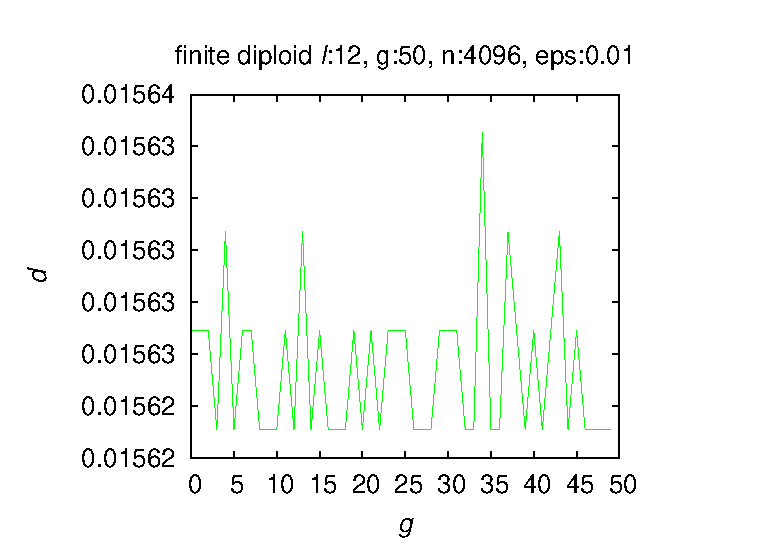
\includegraphics{figures/eps/vio/mu/b12/e0.01/n00004096_fin_dip.eps}}}\hspace{-3em}%
\subfloat{
\resizebox{8cm}{5cm}{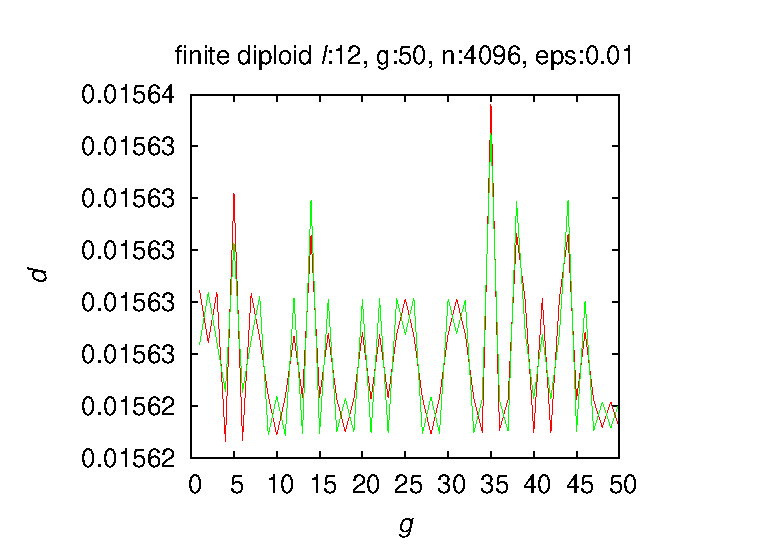
\includegraphics{figures/eps/vio/mu/b12/e0.01/n00004096_fin_dip_wovio.eps}}}\vspace{-1em}  \hspace{-3em}%
\end{center}
\begin{center}
\subfloat{
\resizebox{8cm}{5cm}{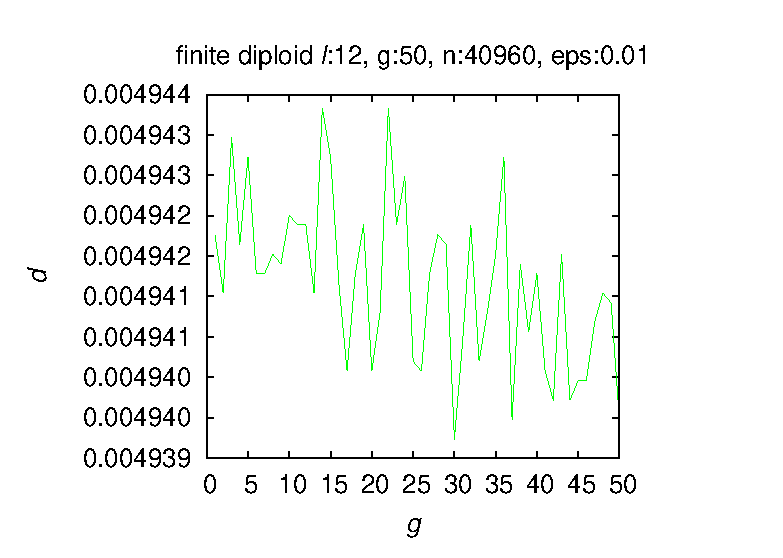
\includegraphics{figures/eps/vio/mu/b12/e0.01/n00040960_fin_dip.eps}}}\hspace{-3em}%
\subfloat{
\resizebox{8cm}{5cm}{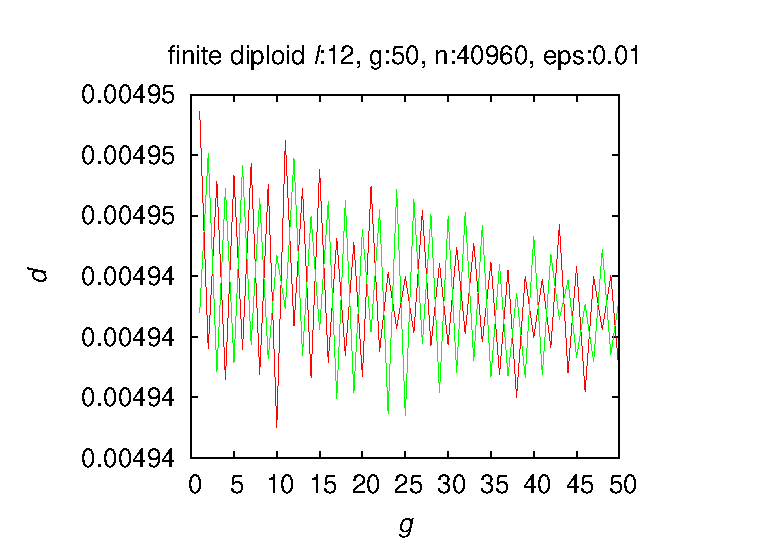
\includegraphics{figures/eps/vio/mu/b12/e0.01/n00040960_fin_dip_wovio.eps}}}\vspace{-1em}  \hspace{-3em}%
\end{center}


\begin{center}
\subfloat{
\resizebox{8cm}{5cm}{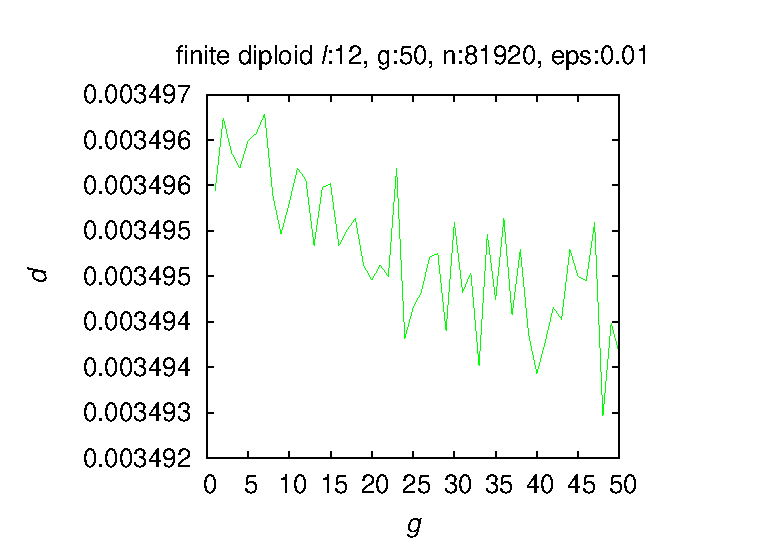
\includegraphics{figures/eps/vio/mu/b12/e0.01/n00081920_fin_dip.eps}}}\hspace{-3em}%
\subfloat{
\resizebox{8cm}{5cm}{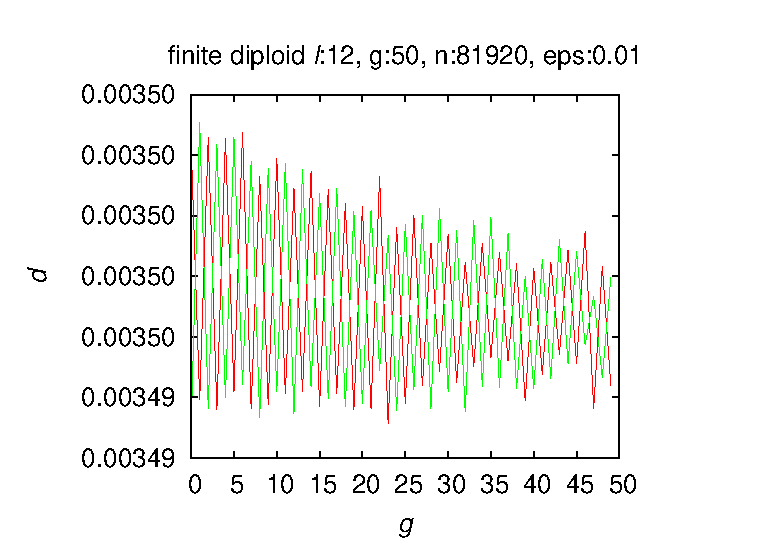
\includegraphics{figures/eps/vio/mu/b12/e0.01/n00081920_fin_dip_wovio.eps}}}\vspace{-1em}  \hspace{-3em}%
\end{center}

\begin{center}
\subfloat{
\resizebox{8cm}{5cm}{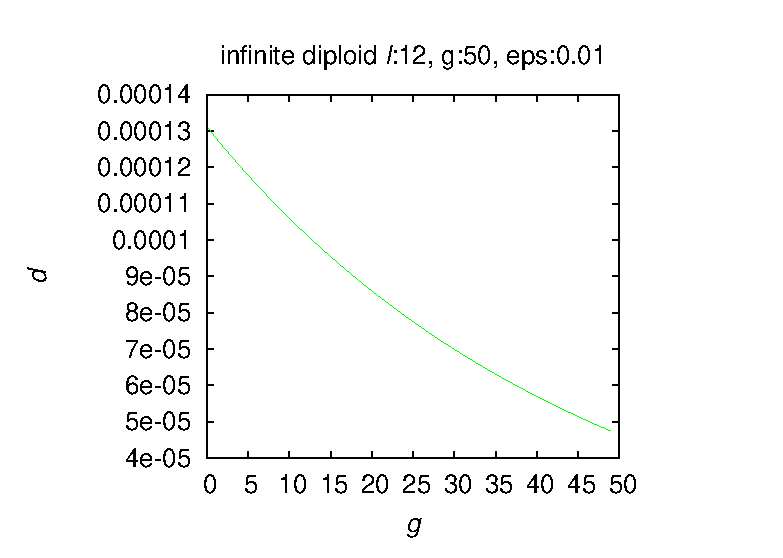
\includegraphics{figures/eps/vio/mu/b12/e0.01/inf_dip.eps}}}\hspace{-3em}%
\subfloat{
\resizebox{8cm}{5cm}{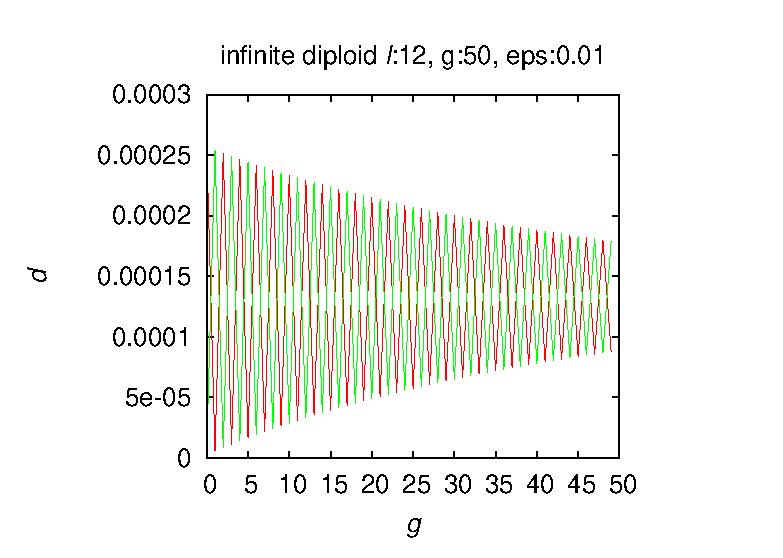
\includegraphics{figures/eps/vio/mu/b12/e0.01/inf_dip_wovio.eps}}}\vspace{-0.5em}  \hspace{-3em}%


\caption{\textbf{Infinite and finite diploid population oscillation behavior in case of violation in $\bm{\mu}$ for genome length $\ell = 12$ and $\bm{\epsilon} = 0.01$:} 
  In left column, $d'$ is distance of finite population of size $n$ or infinite population to limit $\bm{z}^\ast$ for $g$ generations. In right column, $d$ is distance of finite population of size $N$ or infinite population to limits without violation.}
\label{oscillation_12d_vio_mu_0.01}
\end{center}
\end{figure}

% l = 14

\begin{figure}[H]
\begin{center}
\subfloat{
\resizebox{8cm}{5cm}{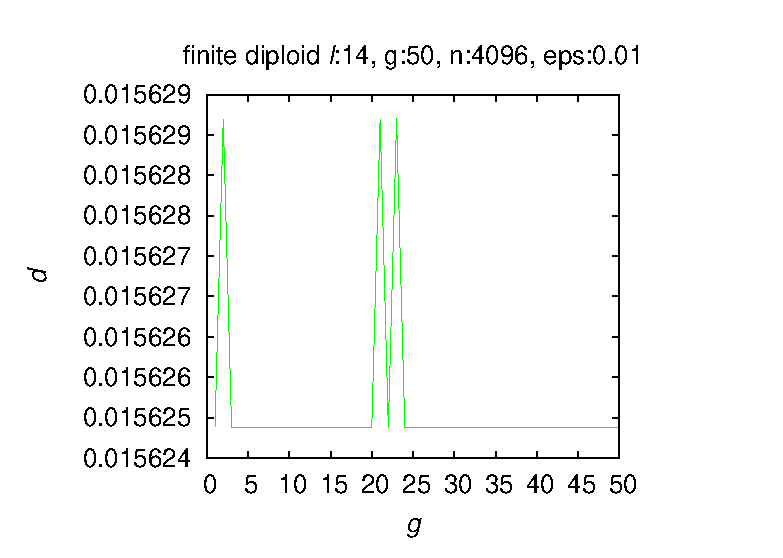
\includegraphics{figures/eps/vio/mu/b14/e0.01/n00004096_fin_dip.eps}}}\hspace{-3em}%
\subfloat{
\resizebox{8cm}{5cm}{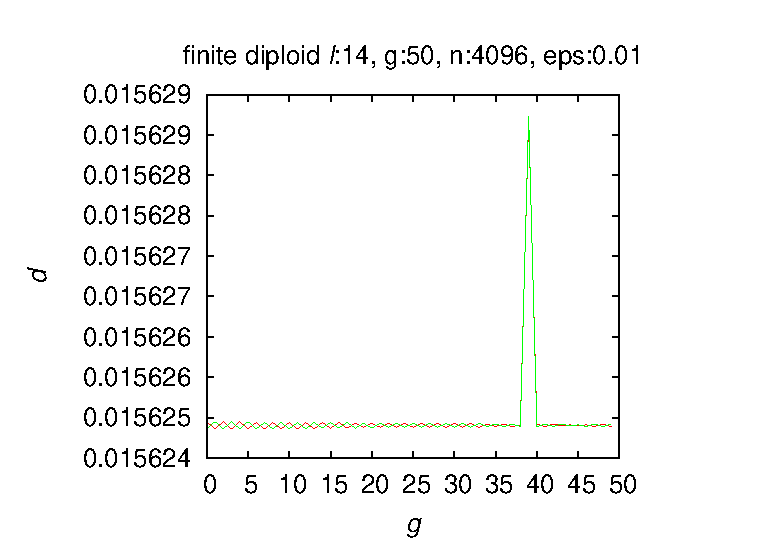
\includegraphics{figures/eps/vio/mu/b14/e0.01/n00004096_fin_dip_wovio.eps}}}\vspace{-1em}  \hspace{-3em}%
\end{center}
\begin{center}
\subfloat{
\resizebox{8cm}{5cm}{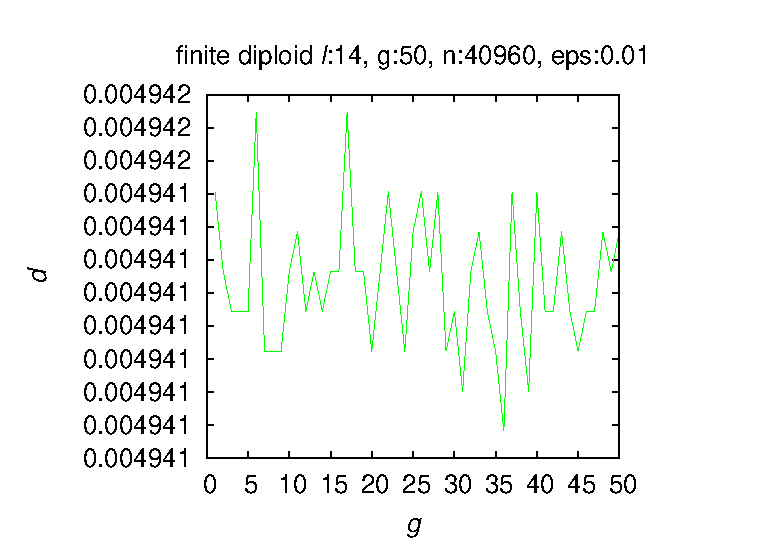
\includegraphics{figures/eps/vio/mu/b14/e0.01/n00040960_fin_dip.eps}}}\hspace{-3em}%
\subfloat{
\resizebox{8cm}{5cm}{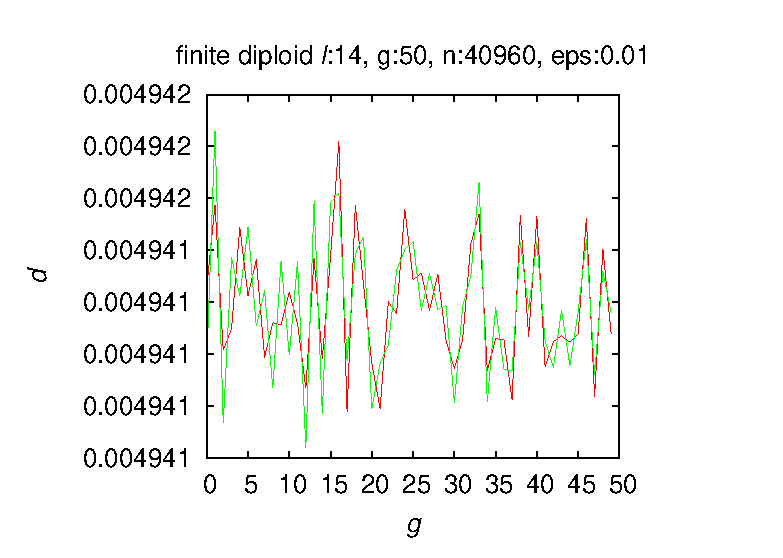
\includegraphics{figures/eps/vio/mu/b14/e0.01/n00040960_fin_dip_wovio.eps}}}\vspace{-1em}  \hspace{-3em}%
\end{center}


\begin{center}
\subfloat{
\resizebox{8cm}{5cm}{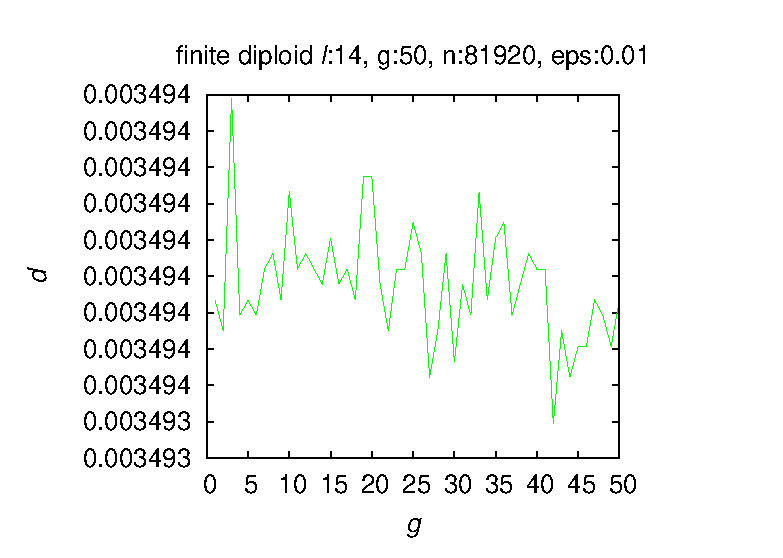
\includegraphics{figures/eps/vio/mu/b14/e0.01/n00081920_fin_dip.eps}}}\hspace{-3em}%
\subfloat{
\resizebox{8cm}{5cm}{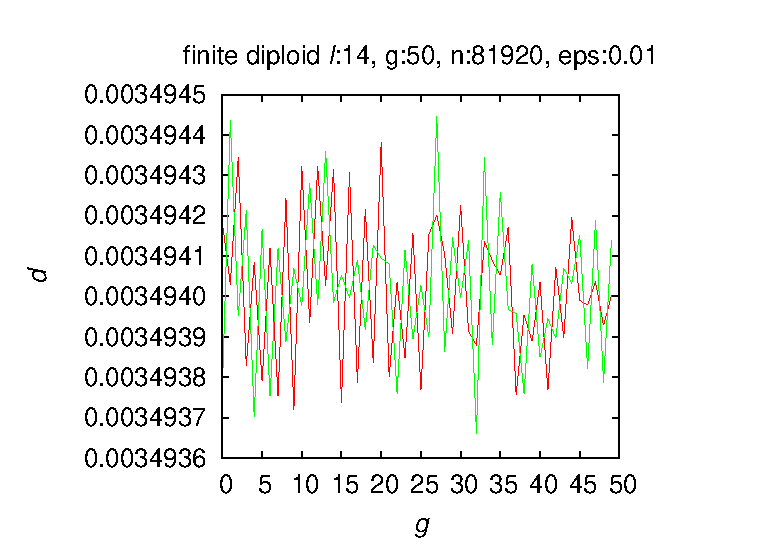
\includegraphics{figures/eps/vio/mu/b14/e0.01/n00081920_fin_dip_wovio.eps}}}\vspace{-1em}  \hspace{-3em}%
\end{center}

\begin{center}
\subfloat{
\resizebox{8cm}{5cm}{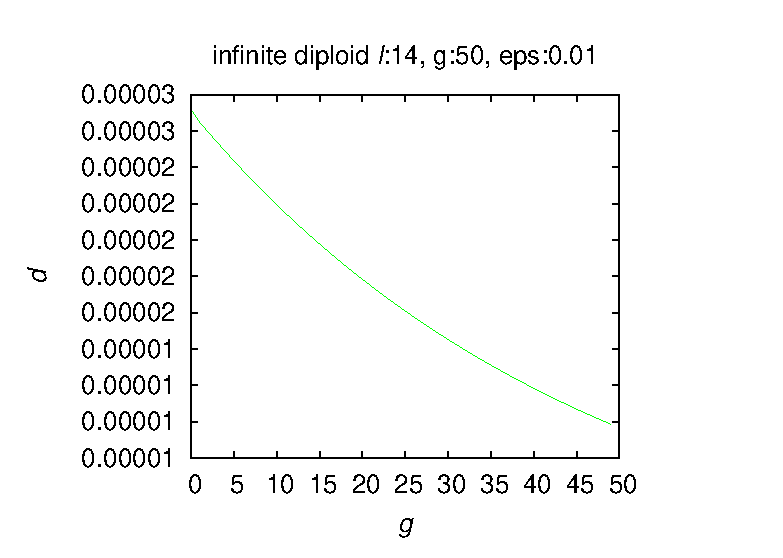
\includegraphics{figures/eps/vio/mu/b14/e0.01/inf_dip.eps}}}\hspace{-3em}%
\subfloat{
\resizebox{8cm}{5cm}{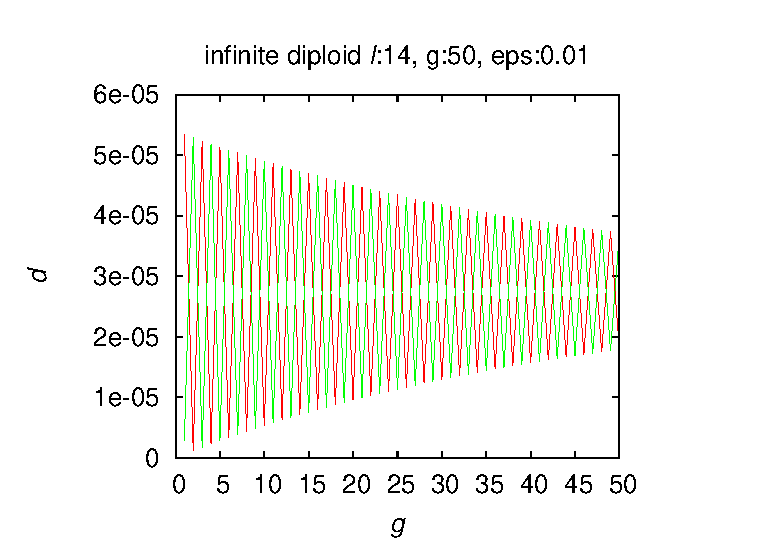
\includegraphics{figures/eps/vio/mu/b14/e0.01/inf_dip_wovio.eps}}}\vspace{-0.5em}  \hspace{-3em}%


\caption{\textbf{Infinite and finite diploid population oscillation behavior in case of violation in $\bm{\mu}$ for genome length $\ell = 14$ and $\bm{\epsilon} = 0.01$:} 
  In left column, $d'$ is distance of finite population of size $n$ or infinite population to limit $\bm{z}^\ast$ for $g$ generations. In right column, $d$ is distance of finite population of size $N$ or infinite population to limits without violation.}
\label{oscillation_14d_vio_mu_0.01}
\end{center}
\end{figure}

The right column in figures \ref{oscillation_8d_vio_mu_0.01} through \ref{oscillation_14d_vio_mu_0.01} 
shows distance of finite and infinite diploid populations to non-violation limits $\bm{p^\ast}$ and $\bm{q^\ast}$ with $\bm{\epsilon} \;=\; 0.01$. 
Graphs in the right column give picture of oscillating behavior of diploid population given violation. 
Both finite and infinite populations oscillate given violation. Like in haploid case, oscillations are sharper. Since value of $\bm{\epsilon}$ 
is very small, damping of ripples is slow. New masks created in mutation distribution with $\bm{\epsilon} \;=\; 0.01$ have very small 
probability of being used during mutation. Infinite population oscillation did not die out completely in 50 generations. As value of $\ell$ 
increases, random drifting and wiggling of finite population occurs for small population size, and oscillation gets better with increase in population size. 
These are noticed more clearly in figures \ref{oscillation_12d_vio_mu_0.01} and \ref{oscillation_14d_vio_mu_0.01}.

The left column of figures \ref{oscillation_8d_vio_mu_0.01} through \ref{oscillation_14d_vio_mu_0.01} 
shows distance of finite and infinite diploid populations to limit $\bm{z^\ast}$ 
(limit with violation in mutation distribution $\bm{\mu}$) when $\bm{\epsilon} \;=\; 0.01$. 
The distance between finite population and limit $\bm{z}^\ast$ (limit with violation in $\bm{\mu}$ distribution) 
decreases as finite population size increases, 
and finite population shows behavior similar to infinite population behavior as finite population reach large number. 
The distance data for diploid population in case of violation in $\bm{\mu}$ distribution 
with $\bm{\epsilon} \;=\; 0.01$ for different finite population size $N$ are tabulated in table \ref{distanceMuDipEps0.01}.

\begin{table}[ht]
\caption{\textbf{Distance measured for violation in $\bm{\mu}$ with $\bm{\epsilon} \;=\; 0.01$ for diploids:} $\ell$ is genome length, 
and average distance between finite and 
infinite populations is tabulated in last three columns.}
\centering
\begin{tabularx}{0.75\textwidth}{ c *{3}{X}}
\toprule
$\ell$ & $N = 4096$ & $N = 40960$ & $N = 81920$ \\
\midrule
8 & 0.0156	&  0.0050	& 0.0035 \\
10 & 0.0156	&  0.0049	& 0.0035 \\
12 & 0.0156	&  0.0049	& 0.0035 \\
14 & 0.0156	&  0.0049	& 0.0035 \\
\bottomrule
\end{tabularx}
\label{distanceMuDipEps0.01}
\end{table}

From table \ref{distanceMuDipEps0.01}, average distance calculated for finite population size $4096$ is $0.0156$, 
for size $40960$ is $0.0049$ and for size $81920$ is $0.0035$. These results show average distance 
between finite population and limit $\bm{z^\ast}$ closely follows expected single step distance 
between finite and infinite population given in \ref{tableExpectedDistance}. The distance decreased as $1/\sqrt{N}$. 
Also, the distance is smaller in diploid populations than in haploid populations with $\bm{\epsilon} \;=\; 0.01$.



